\chapter{Рекуррентный Трансформер с памятью}\label{ch:ch2}

В предыдущей главе~\ref{ch:ch1} обсуждались различные механизмы памяти в нейросетевых архитектурах, в том числе - архитектура Трансформер. Подведем краткий итог по данной архитектуре. 

Трансформеры широко применяются в различных областях и задачах~\cite{RadfordNarasimhanEtAl_2018_Improving_language_understanding_by_generative_pre-training, speech-transformer, devlin2019bert, dosovitskiy2021vit, dalle, jaegle2021perceiverio}. Основой архитектуры трансформера является механизм самовнимания, который обновляет представление каждого элемента последовательности, интегрируя информацию от всех других элементов. Этот подход позволяет создавать насыщенные контекстные представления для каждого элемента к завершению процесса кодирования. В результате модель объединяет в одном представлении как глобальные, так и локальные признаки последовательности. Однако такое смешение двух типов информации создает определенные ограничения. Глобальные признаки распределяются по всем элементам последовательности, что может приводить к их «размытию» и усложнять их извлечение. Еще одним известным недостатком трансформеров является их низкая масштабируемость по длине входной последовательности, что затрудняет обработку длинных данных~\cite{child2019generating, guo2019startransformer, dai2019transformerxl, beltagy2020longformer, ainslie2020encoding, zaheer2020big, wang2020linformer, choromanski2020performer}. Существующие подходы, связанные с упрощением механизма внимания~\cite{katharopoulos2020transformers,beltagy2020longformer,zaheer2020big,ainslie2020encoding}, страдают от деградации качества по сравнению с полноценным Трансформером. 

Рекуррентные модели на уровне сегментов являются перспективной альтернативой трансформерам для работы с длинными контекстами, особенно в условиях ограниченных вычислительных ресурсов. Они характеризуются линейной временной сложностью и постоянным объемом используемой памяти, что делает их подходящими для обработки очень длинных последовательностей. Однако такие модели наследуют проблемы рекуррентных нейронных сетей (RNN), включая узкие места скрытых состояний и сложности с обучением через обратное распространение ошибки во времени (BPTT), которые требуют специализированных решений.

В данной главе рассматривается применение RMT к задачам, которые требуют глобальной информации о всей последовательности, включая копирование, реверсирование и ассоциативное извлечение в условиях сегментированного входа. Хотя и RMT и Transformer-XL хорошо справляются с этими задачами, при увеличении длины последовательности RMT начинает превосходить Transformer-XL. Также эксперименты показэвают, что RMT демонстрирует сопоставимые с Transformer-XL результаты на задачах языкового моделирования, но требует меньше памяти. Код RMT, результаты и гиперпараметры экспериментов доступны в открытом доступе\footnote{\url{https://github.com/booydar/LM-RMT}.}.


\section{Рекуррентный Трансформер с памятью.}


\begin{figure} 
    \centering
    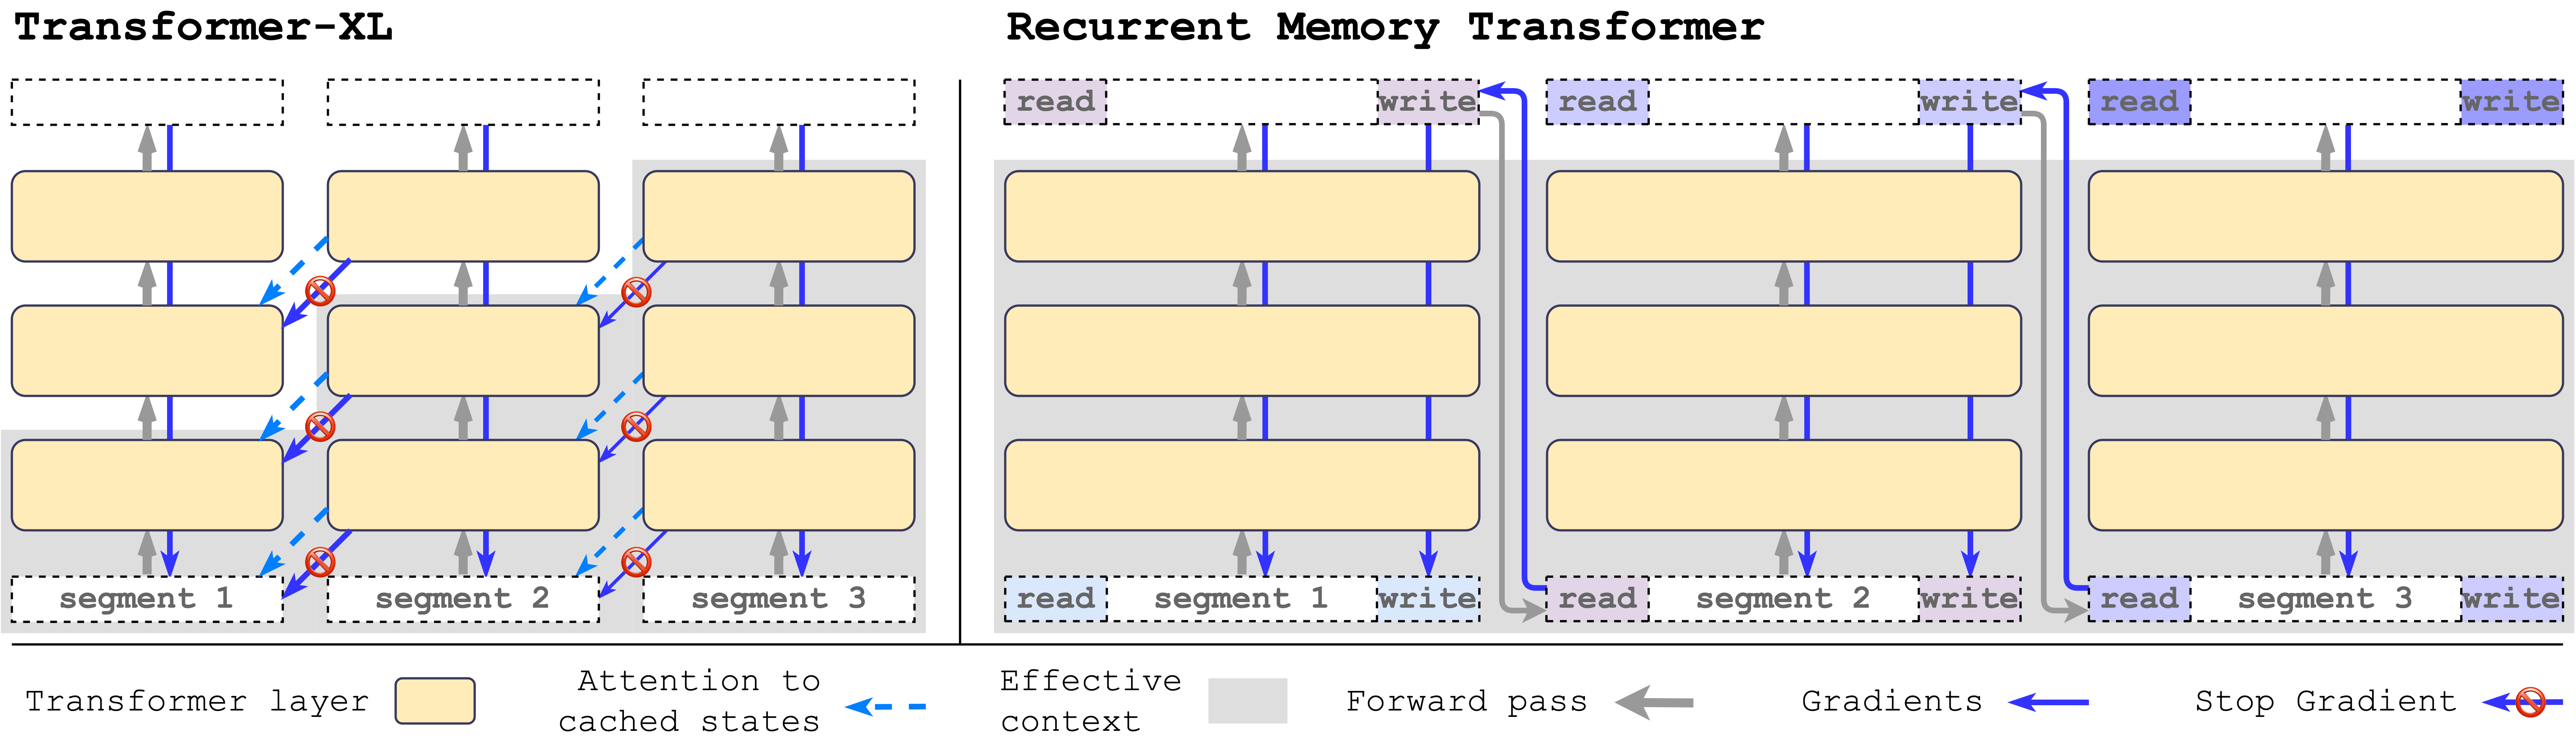
\includegraphics[width=1.0\linewidth]{images/part2/Tr-XL_RMT_full_1.png} 
    \caption{\textbf{Сравнение Recurrent Memory Transformer (RMT) и Transformer-XL.} Архитектура RMT добавляет глобальные токены памяти, которые позволяют реализовать рекуррентность на уровне сегментов. Для операций чтения и записи токены памяти добавляются к входной последовательности; допускается использование нескольких токенов для каждой операции. Обновлённые токены записи передаются следующим сегментам. В отличие от Transformer-XL, где эффективность кеша ограничивается глубиной сети, RMT использует токены памяти для рекуррентности без подобных ограничений. Для обучения RMT применяется BPTT, который обеспечивает распространение градиентов через токены памяти между сегментами.}
    \label{RMT_full} 
\end{figure}

Ряд архитектур, таких как GMAT, ETC и Memory Transformer~\cite{gupta2020gmat, ainslie2020encoding, burtsev2020memory-transformer}, предложили использовать глобальные токены для хранения данных. В Recurrent Memory Transformer в последовательность вводятся специальные токены \texttt{[mem]}, которые обрабатываются вместе с остальными токенами. Каждый токен памяти представлен вектором с вещественными значениями. В начале сегмента к токенам $H_{\tau}^0$ добавляются $m$ токенов памяти, и такие же токены добавляются в конец:

\begin{equation*}
% \begin{gathered}
\tilde{H}^{0}_{\tau} = [H_{\tau}^{mem} \circ H_{\tau}^0 \circ H_{\tau}^{mem}],
\bar{H}^N_\tau = \text{Transformer}(\tilde{H}^{0}_{\tau}),
[H_{\tau}^{read} \circ H_{\tau}^N \circ H_{\tau}^{write}] := \bar{H}^N_\tau,
%\end{gathered}
\end{equation*}
В данном случае $N$ означает количество слоев трансформера.

Обычно такие токены размещаются в начале последовательности, но в архитектурах с каузальным маскированием внимания это мешает сбору информации из последующих токенов. Если же токены памяти располагаются в конце последовательности, они становятся недоступными для предыдущих токенов. Для решения этой проблемы при рекуррентной обработке последовательностей вводится раздельная память для чтения и записи, в начале и конце последовательности соответственно. Представления токенов памяти с конца одного сегмента передаются на вход следующего как в начало, так и в конец.Начальные токены памяти выступают в роли памяти чтения, позволяя токенам входной последовательности обращаться к состояниям памяти, полученным из предыдущего сегмента. Завершающие токены памяти работают как память записи, взаимодействуя со всеми токенами текущего сегмента для обновления хранимых представлений. Таким образом, $H_{\tau}^{write}$ содержит обновленные токены памяти для сегмента $\tau$.

Сегменты входных данных обрабатываются последовательно. Чтобы организовать рекуррентную связь между сегментами, выход токенов памяти текущего сегмента передается на вход следующему сегменту:
\begin{equation*}
\begin{gathered}
H_{\tau+1}^{mem} := H_{\tau}^{write},
\tilde{H}^{0}_{\tau+1} = [H_{\tau+1}^{mem} \circ H_{\tau+1}^0 \circ H_{\tau+1}^{mem}].
\end{gathered}
\end{equation*}


% \subsection{Сравнение RMT с аналогами.}

Память RMT основывается только рекуррентности и глобальных токенах, добавляемых во вход модели. Такой подход позволяет сохранить неизменной архитектуру базовой модели Трансформера и обеспечивает совместимость с любыми моделями из данного семейства. При этом изменения происходят только над входными и выходными данными для модели. В данном разделе рассматриваются обучение архитектуры RMT с нуля, модификация предобученных Трансформеров рассматривается в главе~\ref{ch:ch3}. Реализация RMT построена на основе кода Transformer-XL, а сравнение архитектур представлено в~\cref{RMT_full}.

Механизм памяти в RMT организован иначе, чем в Transformer-XL. Если Transformer-XL хранит $m \times N$ токенов памяти для каждого сегмента, то RMT использует только $m$ токенов. При этом представления памяти из предыдущего сегмента в RMT обрабатываются вместе с токенами текущего сегмента через слои трансформера, что эффективно увеличивает глубину обработки памяти до $\tau \times N$ слоев трансформера. Более того, все токены памяти в блоке чтения/записи имеют доступ ко всем токенам этого же блока. Каузальная маска внимания применяется исключительно к токенам входной последовательности (\cref{fig:mem_operations}(d)).

Обучение RMT осуществляется с использованием метода обратного распространения ошибки во времени (BPTT). В отличие от Transformer-XL, в RMT градиенты передаются через состояния памяти между сегментами во время этапа обратного распространения. Количество предыдущих сегментов, задействованных в BPTT, является гиперпараметром, который варьировался в диапазоне от 0 до 4 в наших экспериментах. Увеличение этого параметра приводит к росту вычислительных затрат и требований к памяти GPU, однако можно применять техники, такие как сохранение контрольных точек градиента, для снижения этих затрат.


\section{Эксперименты на задачах, требующих использования памяти}

\label{sec:experiments}

Проведенные эксперименты были направлены на оценку способности Recurrent Memory Transformer удерживать долгосрочные зависимости в нескольких сегментах входных данных. Первый набор задач включал копирование, реверсирование, ассоциативное извлечение и решение квадратных уравнений. Второй был посвящен языковому моделированию: моделированию на уровне слов для WikiText-103~\cite{merity2017wikitext} и на уровне символов для enwik8~\cite{enwik8}. RMT сравнивался с базовыми моделями Transformer и Transformer-XL.

Имплементация
 RMT была выполнена на базе репозитория Transformer-XL\footnote{\url{https://github.com/kimiyoung/transformer-xl}}. Полный перечень гиперпараметров доступен в нашем репозитории и приложениях. Для обучения RMT на языковому моделировании применялись те же параметры, что и для Transformer-XL. В экспериментах с WikiText-103 использовались 16-слойные трансформеры (10 голов внимания, размерность скрытого состояния 410, размерность внутреннего состояния полносвязного слоя 2100), а для enwik8 — 12-слойные трансформеры (8 голов внимания, размерность скрытого состояния 512, размерность внутреннего состояния полносвязного слоя 2048). Оптимизация выполнялась с помощью Adam~\cite{adam} с линейным расписанием скорости обучения, стартующим с $0.00025$ на 200,000 шагов для WikiText-103 и 400,000 шагов для enwik8. В качестве базового варианта рассматривались модели Transformer-XL с нулевым размером памяти.

Используя данную конфигурацию, нам удалось воспроизвести результаты для моделей Transformer-XL, сопоставимые с оригинальной статьей.


\subsection{Алгоритмические задачи}

Модель Recurrent Memory Transformer (RMT) была протестирована на алгоритмических задачах, требующих обработки всей входной последовательности для получения корректного результата. В рекуррентной архитектуре модель должна сохранять информацию из всех предыдущих сегментов, чтобы делать точные предсказания.

В задаче \textit{Копирование} входная последовательность должна быть воспроизведена дважды после появления специального стартового токена. Для задачи \textit{Реверс} модель должна вопроизвести входную последовательность в обратном порядке. В задаче \textit{Ассоциативное извлечение} входные данные состоят из $N$ пар ключ-значение. Один из ключей выбирается случайным образом, и задача модели — выдать соответствующее значение. Ещё одной задачей является решение квадратных уравнений, где данные задачи включают уравнение, его дискриминант и решение. От модели требуется сгенерировать решение и ответ, причём оценивается только точность итогового ответа.

Для всех задач входные и выходные последовательности разделяются на сегменты, которые обрабатываются моделями поочерёдно. Датасеты для алгоритмических задач были предварительно случайным образом сгенерированы и зафиксированы, что обеспечивало их единообразие во всех экспериментах. Для токенизации использовались символы. Поскольку Transformer-XL и RMT являются Transformer декодировщиками, вычисление ошибки производится исключительно по целевым сегментам последовательности, начиная с токена генерации. %Подробное описание процесса обучения представлено в \cref{app:alg_training_details}.

\subsection{Моделирование языка и обработка естественного языка (NLP)}

Для оценки возможностей языкового моделирования использовались два стандартных бенчмарка: WikiText-103 и enwik8. WikiText-103~\cite{merity2017wikitext} предназначен для моделирования языка на уровне слов и включает 103 миллиона слов из статей английской Википедии. Enwik8~\cite{enwik8} используется для моделирования языка на уровне символов и состоит из первых $10^8$ байт XML-текста из английской Википедии. Размеры словаря токенизаторов составляют 267735 слов для WikiText-103 и 204 символа для enwik8.

RMT сравнивался с Transformer-XL и базовой моделью Transformer, использующей только декодер. Конфигурации моделей и параметры обучения были выбраны в соответствии с описанием в статье Transformer-XL. Длина входного контекста для WikiText-103 была установлена равной 150 токенам, а для enwik8 — 512 символам. Также были проведены эксперименты для проверки способности RMT справляться с долгосрочными зависимостями и рекуррентностью. Для этого количество сегментов увеличивалось, одновременно с уменьшением их размера (50 токенов для WikiText-103 и 128 символов для enwik8). Такие изменения усложняют задачу для RMT, поскольку требуется больше полагаться на память, чем на механизм внимания.

\subsection{Обсуждение и интерпретация результатов экспериментов}

Базовая модель Transformer-XL (Tr-XL) и RMT показывают идеальные результаты при решении задач \textit{Копирование} и \textit{Реверс} в односегментных экспериментах (\cref{fig:algotasks}), где рекуррентность не требуется, так как вся последовательность доступна сразу. Однако, в многосегментных задачах базовая модель демонстрирует ухудшение качества из-за отсутствия возможности передачи информации между сегментами. В то же время, обе модели с памятью успешно передают информацию между сегментами.

\begin{figure}
\vskip -0.1in
\centering
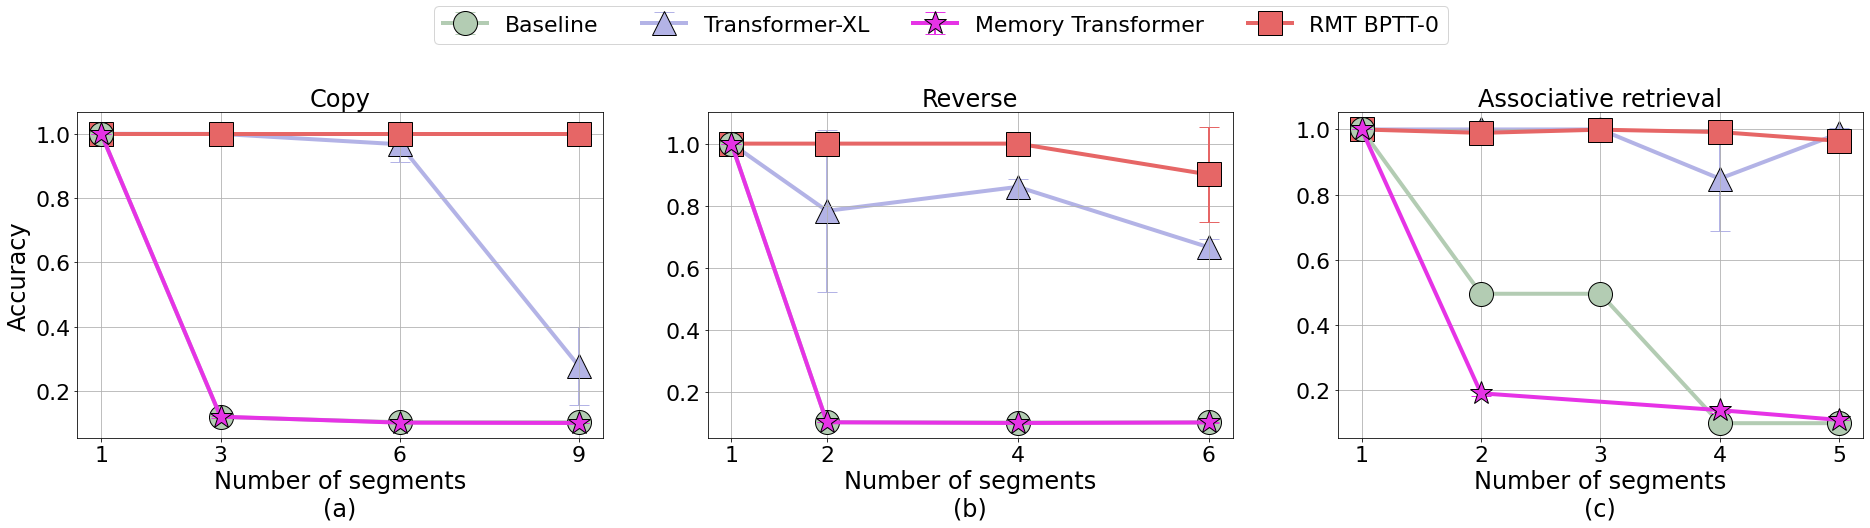
\includegraphics[width=\linewidth]{images/part2/res_combined_updated.png}
\caption{\textbf{RMT показывает лучшую способность к запоминанию с по сравнению с Transformer-XL на алгоритмических задачах при увеличении числа сегментов.} На графиках отображена точность моделей на тестовых данных для задач Копирование, Реверс и Ассоциативное извлечение (слева направо). Размер памяти/кэша для обеих моделей соответствует длине сегмента. В данном эксперименте RMT не передаёт градиенты между сегментами, а результаты базовой модели остаются одинаковыми для всех задач. Длины исходных и целевых последовательностей: 24/48, 24/24 и 10/1 для задач Копирование, Реверс и Ассоциативное извлечение соответственно.}
\label{fig:algotasks}
\end{figure}

В задачах Копирование и Реверс RMT начинает показывать лучшие результаты по сравнению с Transformer-XL, когда число сегментов увеличивается, а памяти становится недостаточно для хранения всех предыдущих токенов. Средняя точность Transformer-XL падает на 0.2 пункта при шести сегментах и достигает уровня базовой модели при девяти сегментах. Похожая тенденция наблюдается в задаче Ассоциативное извлечение, где RMT показывает хорошее качество до четырёх сегментов, как и Transformer-XL. Однако на пяти сегментах точность RMT немного снижается, тогда как у Transformer-XL наблюдается рост средней точности.

Дополнительный анализ изучает влияние количества сегментов, длины последовательности, размера обучающего контекста и памяти на результаты задачи Копирование. По мере увеличения количества сегментов становится всё более важно эффективно передавать информацию между ними. При разбиении последовательности длиной 360 токенов на сегменты (\cref{fig:copy120}) результаты Transformer-XL постепенно ухудшается и в конечном итоге приближается к результатам базовой модели. В то же время, RMT сохраняет идеальную точность. В более сложном эксперименте, где общая длина последовательности увеличена до 720 токенов при фиксированном размере памяти, Transformer-XL быстро теряет точность, а RMT демонстрирует плавное снижение качества (\cref{fig:copy360}).

В задаче решения квадратных уравнений (\cref{tab:quadratic_eq}) базовая модель Transformer без сегментации задаёт верхнюю границу точности. Используя сегментацию и рекуррентность, RMT решает задачу с высокой точностью, тогда как Transformer-XL сталкивается с серьёзными трудностями. 


\begin{table}%[t!]
    \centering
% \footnotesize
% \scalebox{0.5}{
    \begin{tabular}{lccl}
    \toprule
    Model          & memory & segments & $\text{Acc}_{\pm \text{std}}$ \\
    \midrule
    Baseline        &  0           &  1          & 0.99 \tiny{$\pm$ 0.01} \\
    Transformer-XL           &  30          &  6          & 0.93 \tiny{$\pm$ 0.02} \\
    RMT             &  30          &  6          & 0.99 \tiny{$\pm$ 0.002} \\
    \bottomrule
    \end{tabular}
% }

% \vspace{1mm} 
\caption{\textbf{Задача о квадратных уравнениях.} Данная задача включает 180 токенов, представляющих квадратное уравнение, его решение и ответ. Последовательность делится на сегменты, причём последний сегмент содержит ответ. Точность равна 1,0, если предсказанный ответ полностью совпадает с правильным.} 
\label{tab:quadratic_eq} 
\end{table}

Итоги экспериментов по языковому моделированию на уровне слов с использованием корпуса WikiText-103 представлены в \cref{tab:wt103}. При длине сегмента 150 модели Tr-XL и RMT значительно превосходят базовую модель и Memory Transformer (MemTr), что демонстрирует важность увеличения эффективной длины контекста. Этот результат достигается за счёт использования кэша Tr-XL или памяти RMT.

Механизм чтения и записи памяти в RMT более эффективен по сравнению с Memory Transformer. Модели RMT с размерами памяти 10 и 25 показывают схожие результаты с Transformer-XL при размере памяти 75, что свидетельствует о более эффективном использовании памяти в RMT. Более того, меньший размер памяти RMT позволяет снизить требования к объёму памяти GPU.

Для проверки работы с более длинными зависимостями размер сегмента уменьшен до 50, что увеличивает число рекуррентных шагов. В таких условиях RMT с памятью размером 1 демонстрирует результаты, аналогичные Transformer-XL с памятью размером 10. Важно отметить, что память Transformer-XL содержит скрытые состояния всех слоёв (в данном случае $10 \times 16$ векторов), тогда как память RMT ограничивается \textit{memory\_size} векторами. При этом модели Transformer-XL с памятью размером 50 и RMT с памятью размером 5 имеют схожие значения перплексии.% (см. \cref{app:wt103}).

Сочетание RMT с кэшем Tr-XL, где последний используется как краткосрочная память для ближайшего контекста, а RMT — как долгосрочная память, обеспечивает наилучшие результаты на WikiText-103, превосходя отдельную модель Tr-XL.

\begin{table}%[ht] 
% \small
\centering
\fontsize{7}{8}
\selectfont 
\begin{tabular}{lccl}
\toprule
Model          & memory & segment len & $\text{ppl}_{\pm \text{std}}$ \\
\midrule
Tr-XL (paper)   &  150         &  150        & 24.0  \\
\midrule
Baseline        &  0           &  150          & 29.95 \tiny{$\pm$ 0.15} \\
MemTr           &  10          &  150         & 29.63 \tiny $\pm$ 0.06 \\
Tr-XL (ours)    &  150         &  150        & 24.12 \tiny $\pm$ 0.05 \\
\midrule
Tr-XL           &  25          &  150         & 25.57 \tiny $\pm$ 0.02 \\
Tr-XL           &  75          &  150         & \underline{24.68} \tiny $\pm$ 0.01 \\
RMT BPTT-3      &  10          &  150         & 25.04 \tiny $\pm$ 0.07 \\
RMT BPTT-2      &  25          &  150         & \underline{24.85} \tiny $\pm$ 0.31 \\
Tr-XL + RMT
&75+5 &  150        &  24.47 \tiny $\pm$ 0.05 \\
Tr-XL + RMT
&150+10&  150        & \textbf{23.99} \tiny $\pm$ 0.09 \\
\midrule
Baseline        &   0          &  50          & 39.05 \tiny $\pm$ 0.01 \\
Tr-XL           &   100         &  50         & \textbf{25.66} \tiny $\pm$ 0.01 \\
Tr-XL           &   50         &  50         & \underline{26.54} \tiny $\pm$ 0.01 \\
Tr-XL           &   25         &  50         & 27.57 \tiny $\pm$ 0.09\\
Tr-XL           &   10         &  50         & \textit{28.98} \tiny $\pm$ 0.11 \\
RMT BPTT-1      &   1          &  50          & \textit{28.71} \tiny $\pm$ 0.03 \\
RMT BPTT-3      &   10          &  50          & \textit{26.37} \tiny $\pm$ 0.01\\
\bottomrule
\label{tab:wt103}
\end{tabular}
\caption{\textbf{Языковое моделирование на WikiText-103.} В таблице указаны средние значения перплексии для лучших вариаций моделей RMT. Подчёркнуты данные, показывающие схожие результаты моделей Tr-XL и RMT. Модели RMT с меньшими размерами памяти достигают аналогичных результатов, что и модели Tr-XL с большими размерами памяти. Совмещение кэша Tr-XL с памятью RMT показывает наилучшее качество.}
\end{table}



На наборе данных enwik8 модели RMT с памятью размером 5 демонстрируют сопоставимые результаты с моделями Transformer-XL с памятью размером 40. Это подчёркивает способность RMT эффективно использовать ограниченные размеры памяти.% Подробные данные представлены в \cref{app:enwik8}.

Recurrent Memory Transformer (RMT) делает предсказания, анализируя контекст из \texttt{\#BPTT\_unrolls} предыдущих сегментов и текущего сегмента. В то же время Transformer-XL не использует BPTT и опирается только на кэшированные состояния (\texttt{memory\_size}) и текущий сегмент, что формирует общее количество токенов: \texttt{memory\_size} $+$ \texttt{segment\_length}. На \cref{fig:wt103_context} показано сравнение видимого контекста для RMT и Transformer-XL во время обучения.

\begin{figure}
    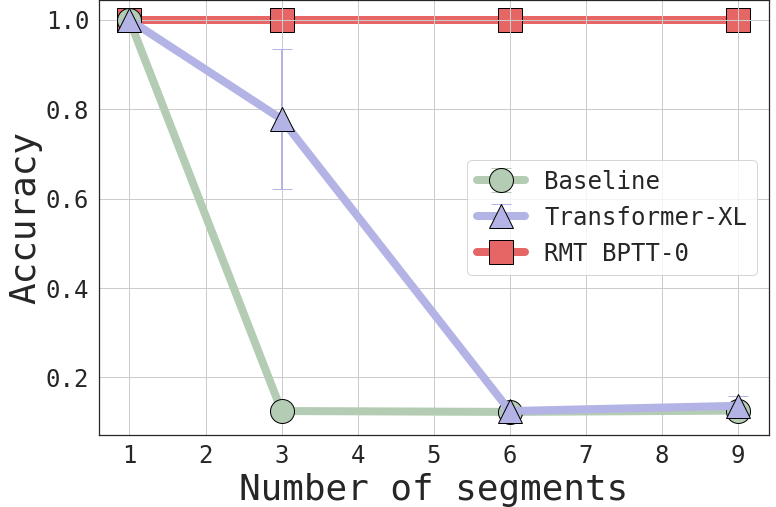
\includegraphics[width=0.4\linewidth]{images/part2/copy120.png}
    \caption{RMT лучше использует фиксированный размер памяти (60 токенов) по сравнению с Transformer-XL при увеличении длины последовательности для копирования. Длина сегмента одинакова для обоих методов (120).}
    \label{fig:copy120}
\end{figure}

\begin{figure}
    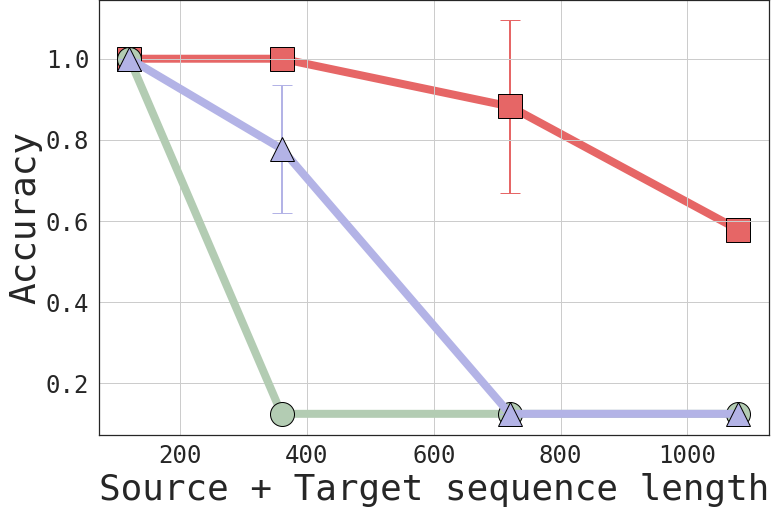
\includegraphics[width=0.4\linewidth]{images/part2/copy120-360.png}
    \caption{RMT успешно решает задачу копирования до 9 сегментов при фиксированной длине последовательности 360, тогда как Transformer-XL не справляется.}
    \label{fig:copy360}
\end{figure}

Обучение моделей RMT с одним вектором памяти позволяет достичь меньшей перплексии, чем у Transformer-XL с размером памяти 10, что говорит о лучшей способности RMT к сжатию информации. Кроме того, модели RMT с памятью 10 и 25 немного уступают Transformer-XL, даже если последний использует больше неконденсированных состояний (50, 100, 200) из предыдущих сегментов. Глубокое распространение градиента на ранние сегменты существенно повышает показатели RMT, подчеркивая значимость метода BPTT. Однако большие размеры памяти и глубокие BPTT приводят к нестабильности обучения и увеличению затрат по GPU-памяти.

Интересно, что добавление одного токена памяти заметно улучшает результаты RMT, но рост этого эффекта замедляется при увеличении памяти с 5 до 50 (\cref{fig:wt103_memory}). Тем не менее, RMT с памятью 5 показывает результаты, сопоставимые с Transformer-XL с кешем 50, что подтверждает способность RMT кодировать компактные представления. Это указывает на существование оптимального размера памяти для RMT, дальнейшее увеличение которого даёт минимальные улучшения.

\begin{figure}
    % \centering
    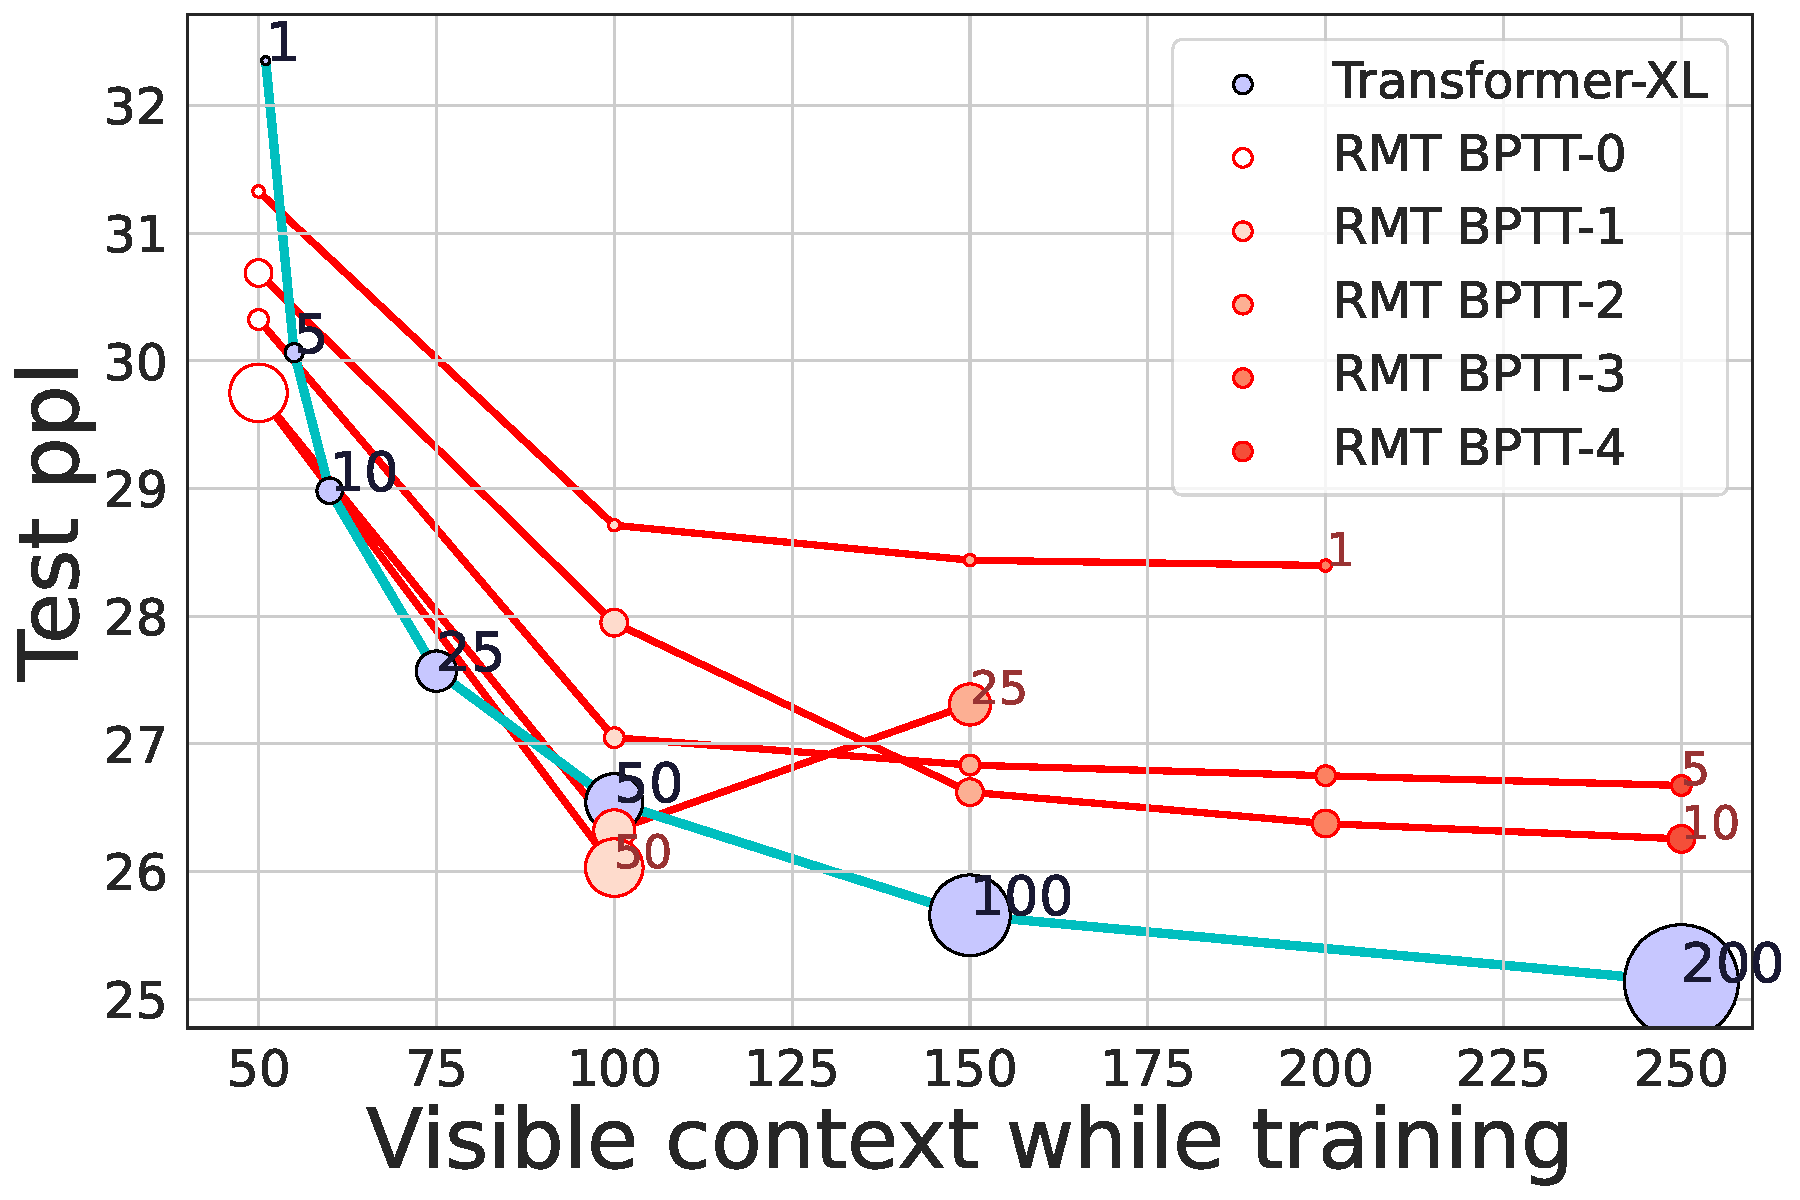
\includegraphics[width=0.4\linewidth]{images/part2/effective_context_50_v1.pdf}
    \caption{Для RMT увеличение видимого контекста на этапе обучения достигается за счёт углубления BPTT, а для Transformer-XL — увеличением кеша. Увеличение видимого контекста уменьшает перплексию для обеих моделей (размер маркера отражает размер памяти).}
    \label{fig:wt103_context}
\end{figure}

\begin{figure}
    % \centering
    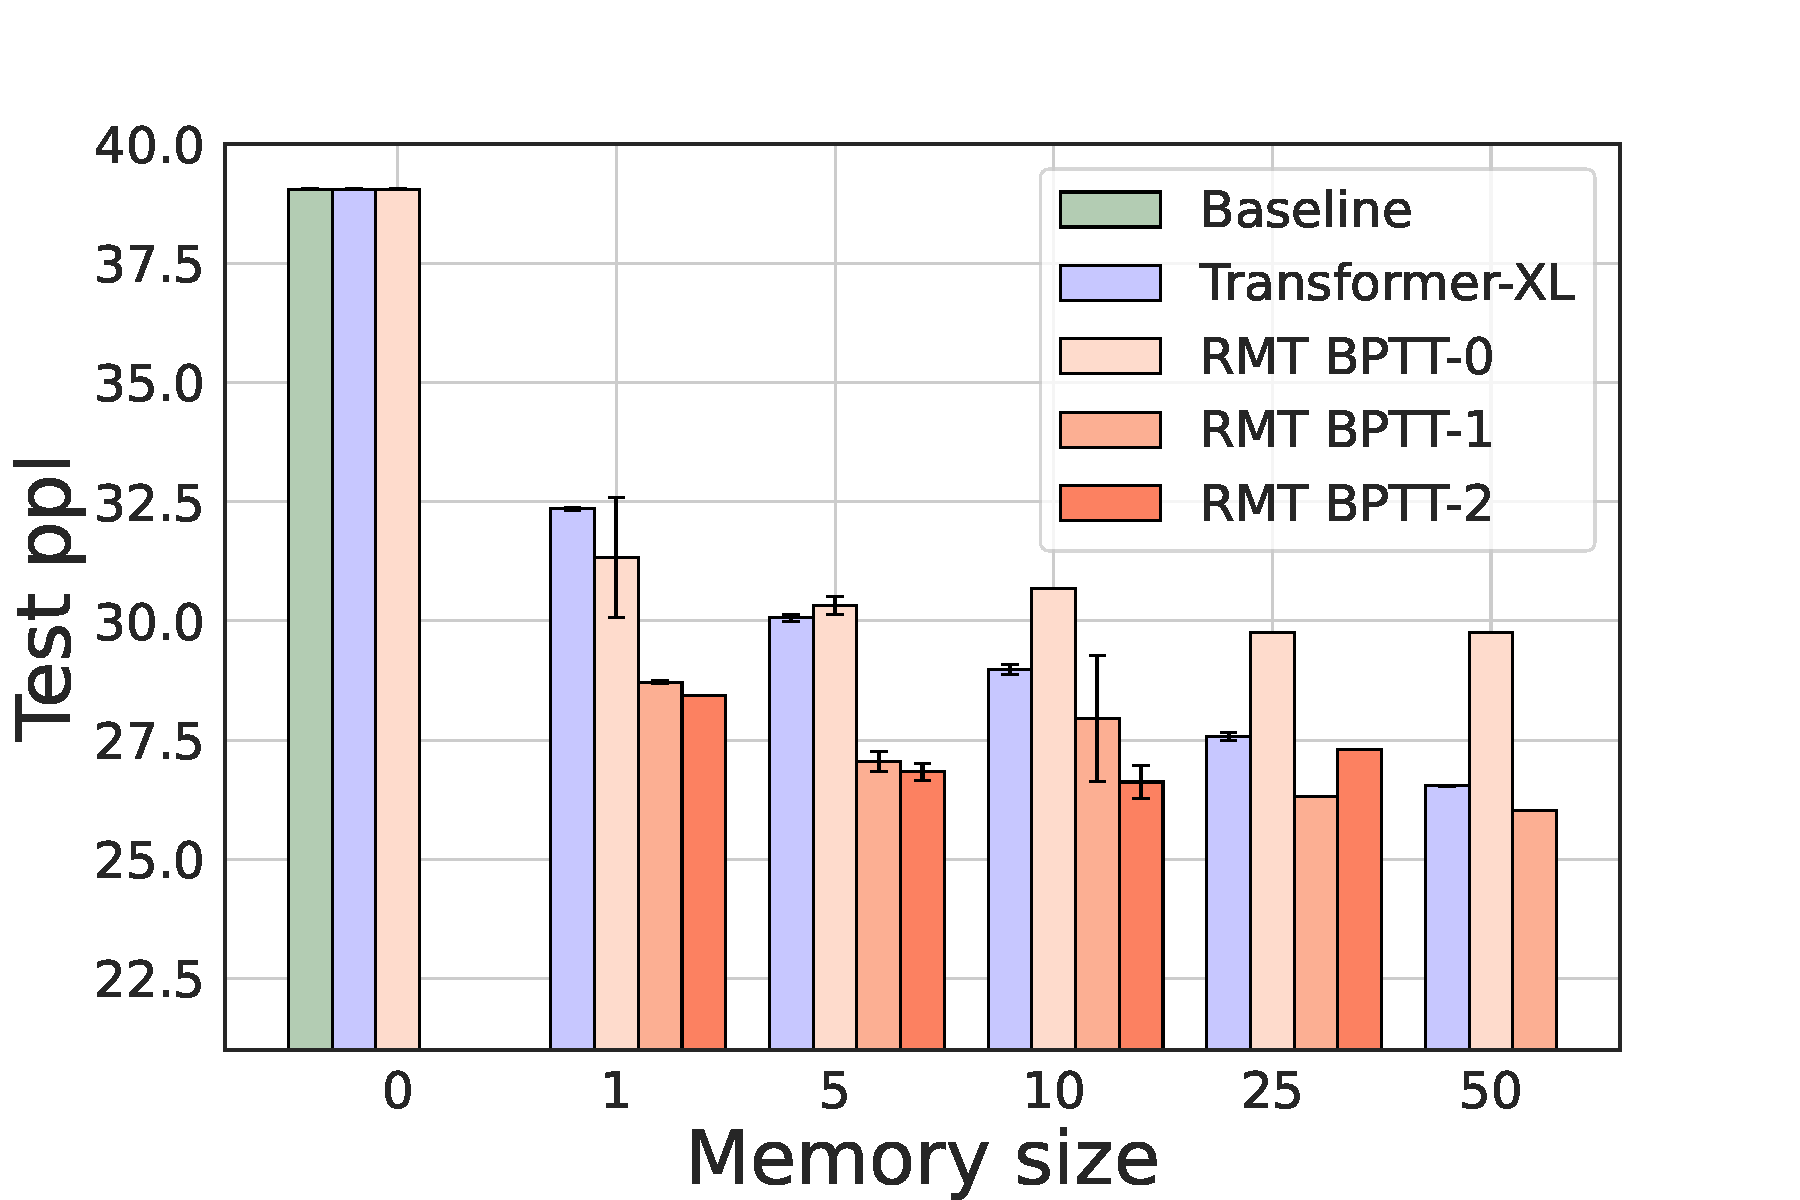
\includegraphics[width=0.4\linewidth]{images/part2/mem_size.pdf}
    \caption{Рекуррентность улучшает результаты RMT по сравнению с Transformer-XL при одинаковых размерах памяти.}
    \label{fig:wt103_memory}
\end{figure}

Для изучения операций с памятью, которые выучивает RMT для решения алгоритмических задач, анализируются карты внимания для задач копирования и реверсирования последовательности, представленные на \cref{fig:mem_operations}. На этих картах перед токенами сегмента расположены токены памяти чтения, соответствующие области в верхнем левом углу, абзац в правом нижнем углу отражены операции между токенами памяти записи. В задаче копирования (\cref{fig:mem_operations}(a), верхняя часть) диагональ в центральной области карты демонстрирует результат операции внимания между токенами последовательности. Дополнительная диагональ в нижней части указывает на последовательную запись токенов в память в исходном порядке. В задаче реверса (\cref{fig:mem_operations}(a), нижняя часть) модель обучается записывать токены в память в обратном порядке, что соответствует логичным ожиданиям.

При воспроизведении целевой последовательности модель извлекает данные из памяти (\cref{fig:mem_operations}(b)) и записывает их в выходную последовательность. Ещё одной ключевой операцией является перезапись памяти (\cref{fig:mem_operations}(c)), когда данные передаются из сегмента чтения памяти в сегмент записи памяти. Эта операция особенно актуальна для RMT в задачах с большим числом сегментов, так как позволяет удерживать информацию о недавних сегментах дольше.

Механизм доступа к памяти Transformer-XL (\cref{fig:mem_operations}(d)) имеет принципиальное отличие. В отличие от RMT, Transformer-XL не поддерживает прямую запись в память без модификации представлений токенов. Его последовательное извлечение памяти из кешированных состояний отображается в виде диагоналей на картах внимания. Использование представлений токенов в качестве памяти снижает эффективность модели в задачах с большим числом сегментов.

% В задаче разворота с четырьмя сегментами Transformer-XL с ограничением памяти до шести (\cref{app:mem_compression}, \cref{fig:mem_compression}(b)) испытывает трудности в управлении представлениями токенов. Модель часто объединяет несколько токенов в одном кешированном состоянии между сегментами, что приводит к средней точности 0.8. В то же время RMT, используя тот же размер памяти, сжимает целые сегменты в токены памяти (\cref{app:mem_compression}, \cref{fig:mem_compression}(a)), достигая идеальной точности 1.

% Визуализация из \cref{fig:mem_operations} и \cref{app:mem_compression} подтверждает, что Transformer-XL объединяет представления предыдущих и текущих сегментов в общих скрытых состояниях для передачи информации. Напротив, выделенные токены памяти в RMT устраняют эту проблему. Способность RMT сжимать последовательности в память дополнительно иллюстрируется в \cref{app:alg_training_details}, \cref{fig:limited_mem}. Для задачи копирования с шестью сегментами RMT сжимает и считывает последовательность из 12 токенов, используя только шесть токенов памяти. При этом уменьшение размера памяти в Transformer-XL значительно снижает точность модели при увеличении числа сегментов более двух.

\begin{figure} 
\centering 
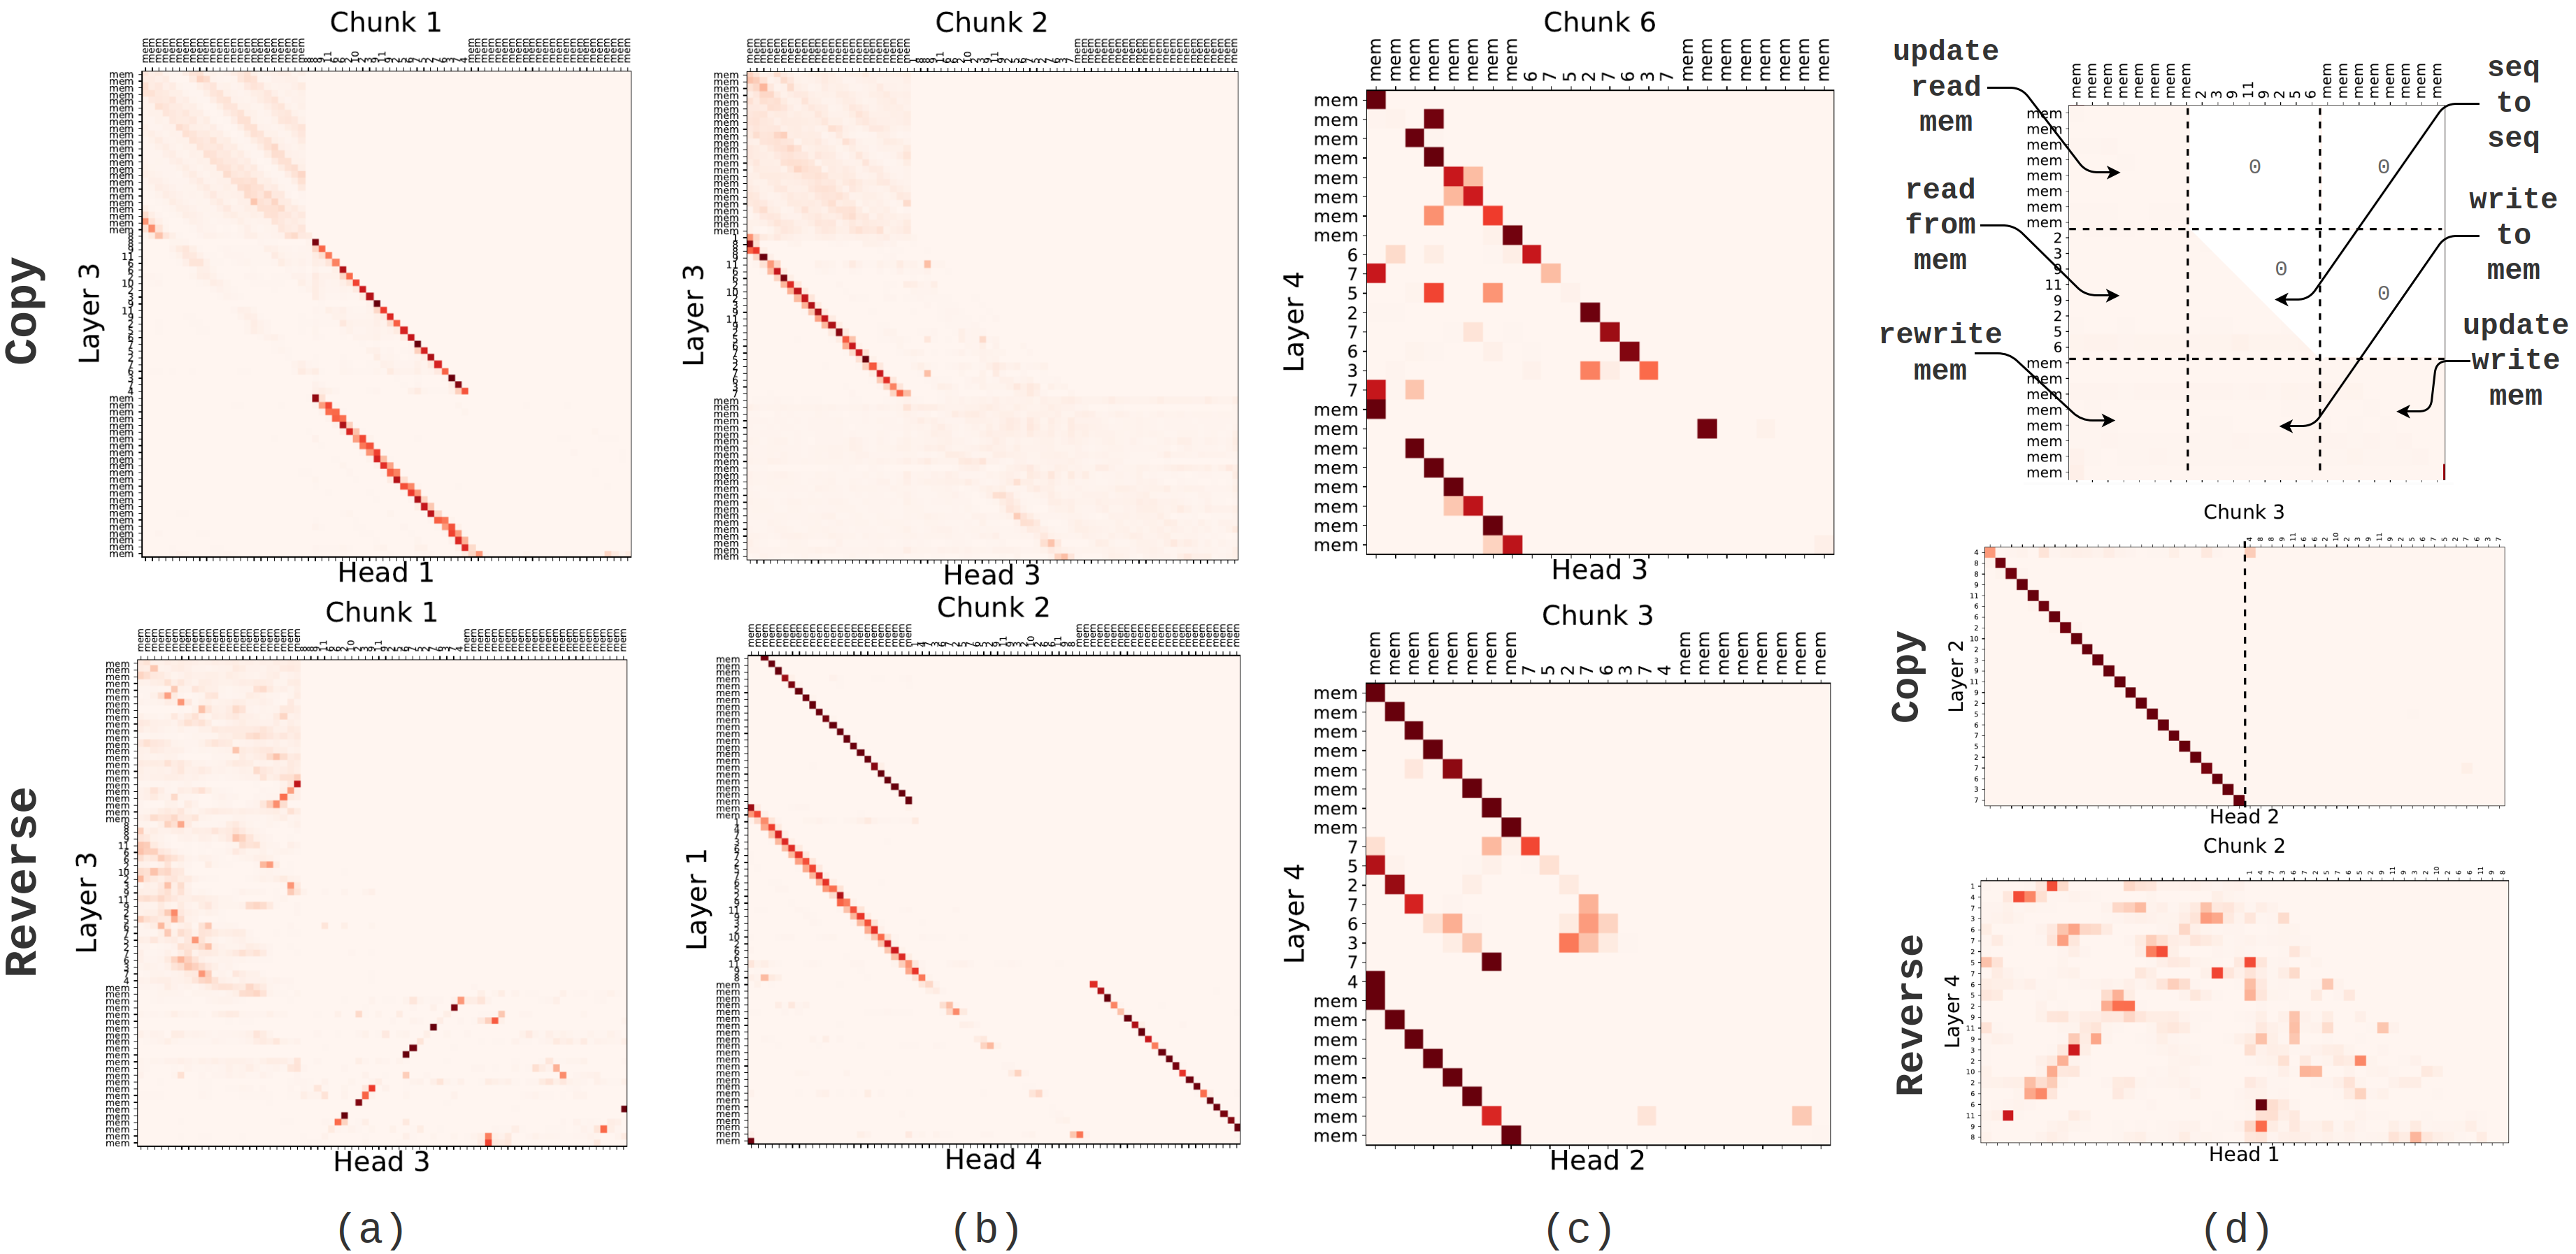
\includegraphics[width=\linewidth]{images/part2/mem_operations.png} 
\caption{\textbf{Тепловые карты внимания для моделей памяти.} (Интенсивность цвета отражает значения внимания.) RMT, длина сегмента = 24, размер памяти = 24: (a) запись в память, (b) чтение из памяти. (c) RMT, длина сегмента = 8, размер памяти = 8: перезапись из чтения памяти в запись памяти. (d) Transformer-XL, длина сегмента = 24, размер памяти = 24: чтение из предыдущих скрытых состояний.} 
\label{fig:mem_operations} 
\end{figure}


\section{Выводы}

В данном разделе был рассмотрен Recurrent Memory Transformer (RMT), представляющий собой простое улучшение модели Transformer с использованием рекуррентной памяти. Модель расширяет входные последовательности специальными глобальными токенами памяти и применяет рекуррентность на уровне сегментов. Это позволяет обучать более компактные представления последовательностей и повышать качество существующих предварительно обученных моделей без значительных дополнительных затрат на вычисления, что делает данный подход более энергоэффективным и экологичным для машинного обучения.

В ходе экспериментов RMT был сравнен с базовым Transformer и Transformer-XL, популярной модификацией Transformer для длинных последовательностей. Модель RMT практически идеально выполняет задачи Копирования, Реверсирования и решения квадратных уравнений на последовательностях, состоящих из нескольких сегментов, превосходя Transformer-XL. Для задачи ассоциативного поиска RMT показал результаты, сопоставимые с Transformer-XL, в то время как базовая версия Transformer оказалась неспособной решать такие задачи в условиях многосегментного разделения.

При обучении в качестве языковой модели RMT демонстрирует значительно лучшие результаты по сравнению с базовым Transformer и достигает уровня качества Transformer-XL при уменьшении размера памяти в 10 раз. Эксперименты также показали, что при фиксированном размере памяти увеличение количества сегментов, для которых выполняется обратное распространение градиентов, приводит к улучшению результатов RMT. Этот подход к дополнению памяти отличается универсальностью и легко адаптируется к другим моделям, основанным на Transformer. Например, сочетание RoBERTa и RMT позволило достичь лидирующих результатов в задаче классификации длинных текстов.

Анализ карт внимания показывает, что повышенная эффективность RMT связана с более рациональным использованием выделенных токенов памяти для хранения представлений входных данных по сравнению с их смешанным хранением в Transformer-XL. Более того, объединение RMT с механизмом кеширования Transformer-XL позволяет превзойти каждую из моделей.

% В целом, Recurrent Memory Transformer представляет собой многообещающую архитектуру для задач, где требуется обучение долгосрочных зависимостей и обработка данных в памяти, таких как алгоритмические задачи и рассуждения. Кроме того, RMT открывает перспективы для интеграции памяти и рекуррентности в другие модели семейства Transformer.


